\documentclass[oneside,10pt]{book}

\usepackage{cdtBook}
\usepackage{usecases}
\usepackage{requerimientos/requisitos}
\usepackage{amsmath}
\usepackage{amssymb}
\usepackage{booktabs}
\usepackage{hyperref}
\usepackage{enumerate}
\usepackage{mensajes/msg_style}
\usepackage{pdfpages} %Para cargar pdfs
\usepackage{estilos/estilos}
%\overfullrule=2cm

%\title{Análisis}
%\subtitle{}
%\author{Autores: \\Fernández Quiñones Isaac\\Huerta Martínez Jesús Manuel\\Pérez García José David}
%\organization{Escuela Superior de Cómputo, IPN}

%%%%%%%%%%%%%%%%%%%%%%%%%%%%%%%%%%%%%%%%%%%%%%%%%%%%%%%%%%%%%%%%
\begin{document}


\includepdf[pages=1]{portada/posible_portada}

%Para cambiar entre portadas comentar la linea anterior y descomentar hasta \end{titlepage}
%\begin{titlepage}
%
%\begin{table*}[htb]
%	\begin{tabular}{p{0.2\textwidth} p{0.7\textwidth}}
%		$ $ \newline%Para que la sigueinte columna empiece en la parte superior
%		
\includegraphics[width=0.2\textwidth]{images/ipn}\par\raggedright
%		\hspace{0.5cm}\rule{0.5mm}{500pt}%
%		\hspace{1cm}\rule{1mm}{500pt}%
%		\hspace{1cm}\rule{0.5mm}{500pt}%
%		&
%	    \vspace{0pt}{\centering\scshape\fontsize{25}{27}\selectfont Instituto Politécnico Nacional\par}
%	    \hspace{0.48cm}\rule{300pt}{1mm}
%	    \vspace{3pt}
%		\hspace{0.48cm}\rule{300pt}{0.5mm}%
%	    \vspace{1cm}
%		{\centering\scshape\fontsize{20}{22}\selectfont Escuela Superior de Cómputo\par}
%		\vspace{1.5cm}
%		{\centering\scshape\fontsize{18}{20}\selectfont ESCOMobile\par}
%		\vspace{1.5cm}
%		{\centering\scshape\fontsize{20}{22}\selectfont \textbf{REPORTE DE TRABAJO TERMINAL}\par}
%		\vspace{1cm}
%		{\centering\scshape\fontsize{16}{18}\selectfont COMO REQUISITO PARA OBTENER EL TÍTULO DE\par}
%		\vspace{10pt}
%		{\centering\scshape\fontsize{18}{20}\selectfont \textbf{Ingeniero en Sistemas Computacionales}\par}
%		\vspace{20pt}
%		{\centering\scshape\fontsize{14}{16}\selectfont PRESENTAN:\par}
%		{\centering\scshape\fontsize{14}{16}\selectfont \textbf{Fernández Quiñones Isaac}\par}
%		{\centering\scshape\fontsize{14}{16}\selectfont \textbf{Huerta Martínez Jesús Manuel}\par}
%		{\centering\scshape\fontsize{14}{16}\selectfont \textbf{Pérez García José David}\par}
%			
%		\vspace{30pt}
%		{\centering\scshape\fontsize{14}{16}\selectfont Directores:\par}
%		{\centering\scshape\fontsize{14}{16}\selectfont \textbf{M en C. Vélez Ulises}\par}
%		{\centering\scshape\fontsize{14}{16}\selectfont \textbf{M en C. Luna Benoso Benjamin}\par}
%		\vfill
%		%Bottom of the page
%		\vspace{20pt}
%		{\centering\scshape\fontsize{14}{16}\selectfont \today \par}\\
%		%{\large \today\par}\\
%	\end{tabular}
%\end{table*}
%
%\end{titlepage}


%\maketitle
%\thispagestyle{empty}
\frontmatter
\tableofcontents
\listoffigures
\listoftables
\mainmatter

%=========================================================
%                                                         INTRODUCCIÓN.
%=========================================================

\chapter{Introducción}

% Introducción.
\cfinput{intro/Introduccion}
% Justificación.
\cfinput{intro/Justificacion}
% Objetivos.
\cfinput{intro/Objetivos}

%=========================================================
%                                                      ESTADO DEL ARTE.
%=========================================================

\chapter{Estado del arte}
\cfinput{estado_arte/estadoarte}

%=========================================================
%                                                       MARCO TEÓRICO.
%=========================================================

\chapter{Marco Teórico}
\cfinput{marco_teorico/marco_teorico}

%=========================================================
%                                                 TÉRMINOS DEL NEGOCIO.
%=========================================================

\chapter{Términos del negocio}
\cfinput{marco_teorico/glosario}

%=========================================================
%                                                            REQUISITOS.
%=========================================================

\chapter{Requisitos de software}
\cfinput{requerimientos/requisitos}

%=========================================================
%                                                 TECNOLOGÍAS A USADAS.
%=========================================================

\chapter{Tecnologías Usadas}
\cfinput{requerimientos/tecnologias}

%=========================================================
%                                                   ANALISIS DE RIESGOS.
%=========================================================

\chapter{Analisis de Riesgos}
\cfinput{riesgos/analisisderiesgos}

%=========================================================
%                                                     REGLAS DE NEGOCIO.
%=========================================================

\chapter{Modelo de Negocios}
\cfinput{reglas_negocio/reglas}

%=========================================================
%                                                         CASOS DE USO.
%=========================================================

% Descripción de casos.
\chapter{Descripción de los casos de uso}
\cfinput{cu_temp/cu_temp}

% Modelado de casos.
\chapter{Modelo de Casos de Uso}
\noindent
Esta sección aborda el modelado de los casos de uso previamente descritos que conformarán la aplicación ESCOMobile. Aquí se detalla la información referente a cada Caso de Uso, sus características como, resumen, propósitos, entradas, salidas, etc., así como las trayectorias principal y alternativas que en los casos se contemplan. 

% Módulo de acceso. 
\cfinput{cu/EM-Acceso/CU01}
\cfinput{cu/EM-Acceso/CU02}
\cfinput{cu/EM-Acceso/CU03}
\cfinput{cu/EM-Acceso/CU04}
\cfinput{cu/EM-Acceso/CU05}
\cfinput{cu/EM-Acceso/CU06}

% Módulo de Mapa.
\cfinput{cu/EM-Mapa/CU01}
\cfinput{cu/EM-Mapa/CU02}

% Módulo de Alumno.
\cfinput{cu/EM-Alumno/CU1}
\cfinput{cu/EM-Alumno/CU1_1}

% Módulo de AlumnoBolsa.
\cfinput{cu/EM-AlumnoBolsa/CU1}
\cfinput{cu/EM-AlumnoBolsa/CU1_1}

% Módulo de AlumnoProfesor. 
\cfinput{cu/EM-AlumnoProfesor/CU1}
\cfinput{cu/EM-AlumnoProfesor/CU1_1}
\cfinput{cu/EM-AlumnoProfesor/CU1_1_1}
\cfinput{cu/EM-AlumnoProfesor/CU1_1_2}
\cfinput{cu/EM-AlumnoProfesor/CU1_1_3}

%\cfinput{cu/EM-Profesor/CU001}
%\cfinput{cu/EM-Profesor/CU005}
%

%\cfinput{cu/EM-WebBolsa/CU002}
%\cfinput{cu/EM-WebBolsa/CU007}
%\cfinput{cu/EM-WebBolsa/CU009}
%\cfinput{cu/EM-WebBolsa/CU010}
%\cfinput{cu/EM-WEB/CU03}
%cfinput{cu/EM-WEB/CU4}

% AlumnoProfesor. 
%\cfinput{cu/EM-AlumnoProfesor/CU1}
%\cfinput{cu/EM-AlumnoProfesor/CU1_1}
%\cfinput{cu/EM-AlumnoProfesor/CU1_1_1}
%\cfinput{cu/EM-AlumnoProfesor/CU1_1_2}
%\cfinput{cu/EM-AlumnoProfesor/CU1_1_3}
%\cfinput{cu/EM-AlumnoProfesor/CU1_1_4}
%\cfinput{cu/EM-AlumnoProfesor/CU1_1_5}

% Bolsa de Trabajo Alumno.
%\cfinput{cu/EM-AlumnoBolsa/CU1}
%\cfinput{cu/EM-AlumnoBolsa/CU1_1}

% Bolsa de trabajo Web. 
%\cfinput{cu/EM-BolsaWeb/CU1}
%\cfinput{cu/EM-BolsaWeb/CU1-1}
%\cfinput{cu/EM-BolsaWeb/CU1-2}
%  /\cfinput{cu/EM-BolsaWeb/CU1-3}
%\cfinput{cu/EM-BolsaWeb/CU1-4}
%\cfinput{cu/EM-BolsaWeb/CU2}
%\cfinput{cu/EM-BolsaWeb/CU3}
%\cfinput{cu/EM-BolsaWeb/CU4}
%\cfinput{cu/EM-BolsaWeb/CU4_1}
%\cfinput{cu/EM-BolsaWeb/CU4_2}
%\cfinput{cu/EM-BolsaWeb/CU4_3}

%\cfinput{cu/EM-Citas/CU01}

%\cfinput{cu/EM-Citas/CU01}
%\cfinput{cu/EM-Citas/CU04}

%=========================================================
%                                                    MODELO DE INTERACCION
%=========================================================

\chapter{Modelo de la Interacción}

\noindent
En este apartado se muestran las diferentes pantallas que componen a la aplicación ESCOMobile,
la forma en que éstas se estructuran y la descripción de las diferentes secciones que las componen.
La información que se puede consultar en la descripción incluye: objetivo, descripción del diseño, 
una imagen que ilustra el diseño descrito, las entradas requeridas (de ser el caso) y las salidas
generadas y mostradas dentro de la propia pantalla, así como los comandos y mensaje con las que
éstas pueden llegar a contar.

\noindent
\newline
A continuación, se muestra la descripción de cada una de las pantallas que forman ESCOMobile,
en el mismo orden del cual se descibieron los casos de uso.

% Pantallas.
\cfinput{Pantallas/Acceso/UI_Acceso}
\cfinput{Pantallas/Mapa/UI_Mapa}
\cfinput{Pantallas/Alumno/UI_Alumno}
\cfinput{Pantallas/AlumnoBolsa/UI_AlumnoBolsa}
\cfinput{Pantallas/AlumnoProfesor/UI_AlumnoProfesor}

%\cfinput{Pantallas/Citas/UI_Citas}
%\cfinput{Pantallas/BolsaWeb/UI_WebBolsa}



%=========================================================
%                                                                MENSAJES.
%=========================================================
\chapter{Modelo de mensajes}
\cfinput{mensajes/mensajes}

%=========================================================
%                                                     MAPAS DE NAVEGACION.
%=========================================================

\chapter{Mapa de navegacion}

	\begin{figure}[htbp!]
		\centering
			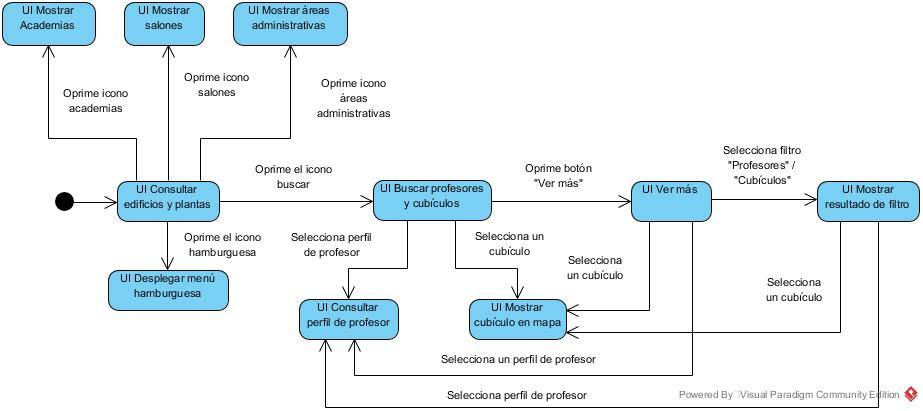
\includegraphics[width=.5\textwidth]{mapa_nave/imagenesnav/buscar1}
		%\caption{Diseño de la Base de Datos.}
		\caption{navegacion Buscar.}
	\end{figure}
	
	\begin{figure}[htbp!]
		\centering
			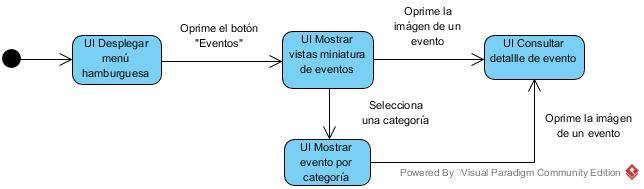
\includegraphics[width=.5\textwidth]{mapa_nave/imagenesnav/eventos}
		%\caption{Diseño de la Base de Datos.}
		\caption{navegacion eventos.}
	\end{figure}
	
	\begin{figure}[htbp!]
		\centering
			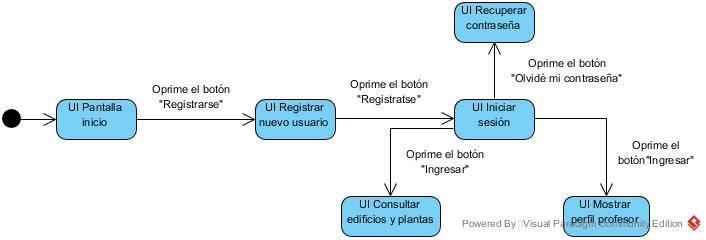
\includegraphics[width=.5\textwidth]{mapa_nave/imagenesnav/registro}
		%\caption{Diseño de la Base de Datos.}
		\caption{navegacion registro.}
	\end{figure}

%=========================================================
%                                                     DOMINIO DEL PROBLEMA.
%=========================================================

\chapter{Modelo del Dominio del problema}

	\begin{figure}[htbp!]
		\centering
			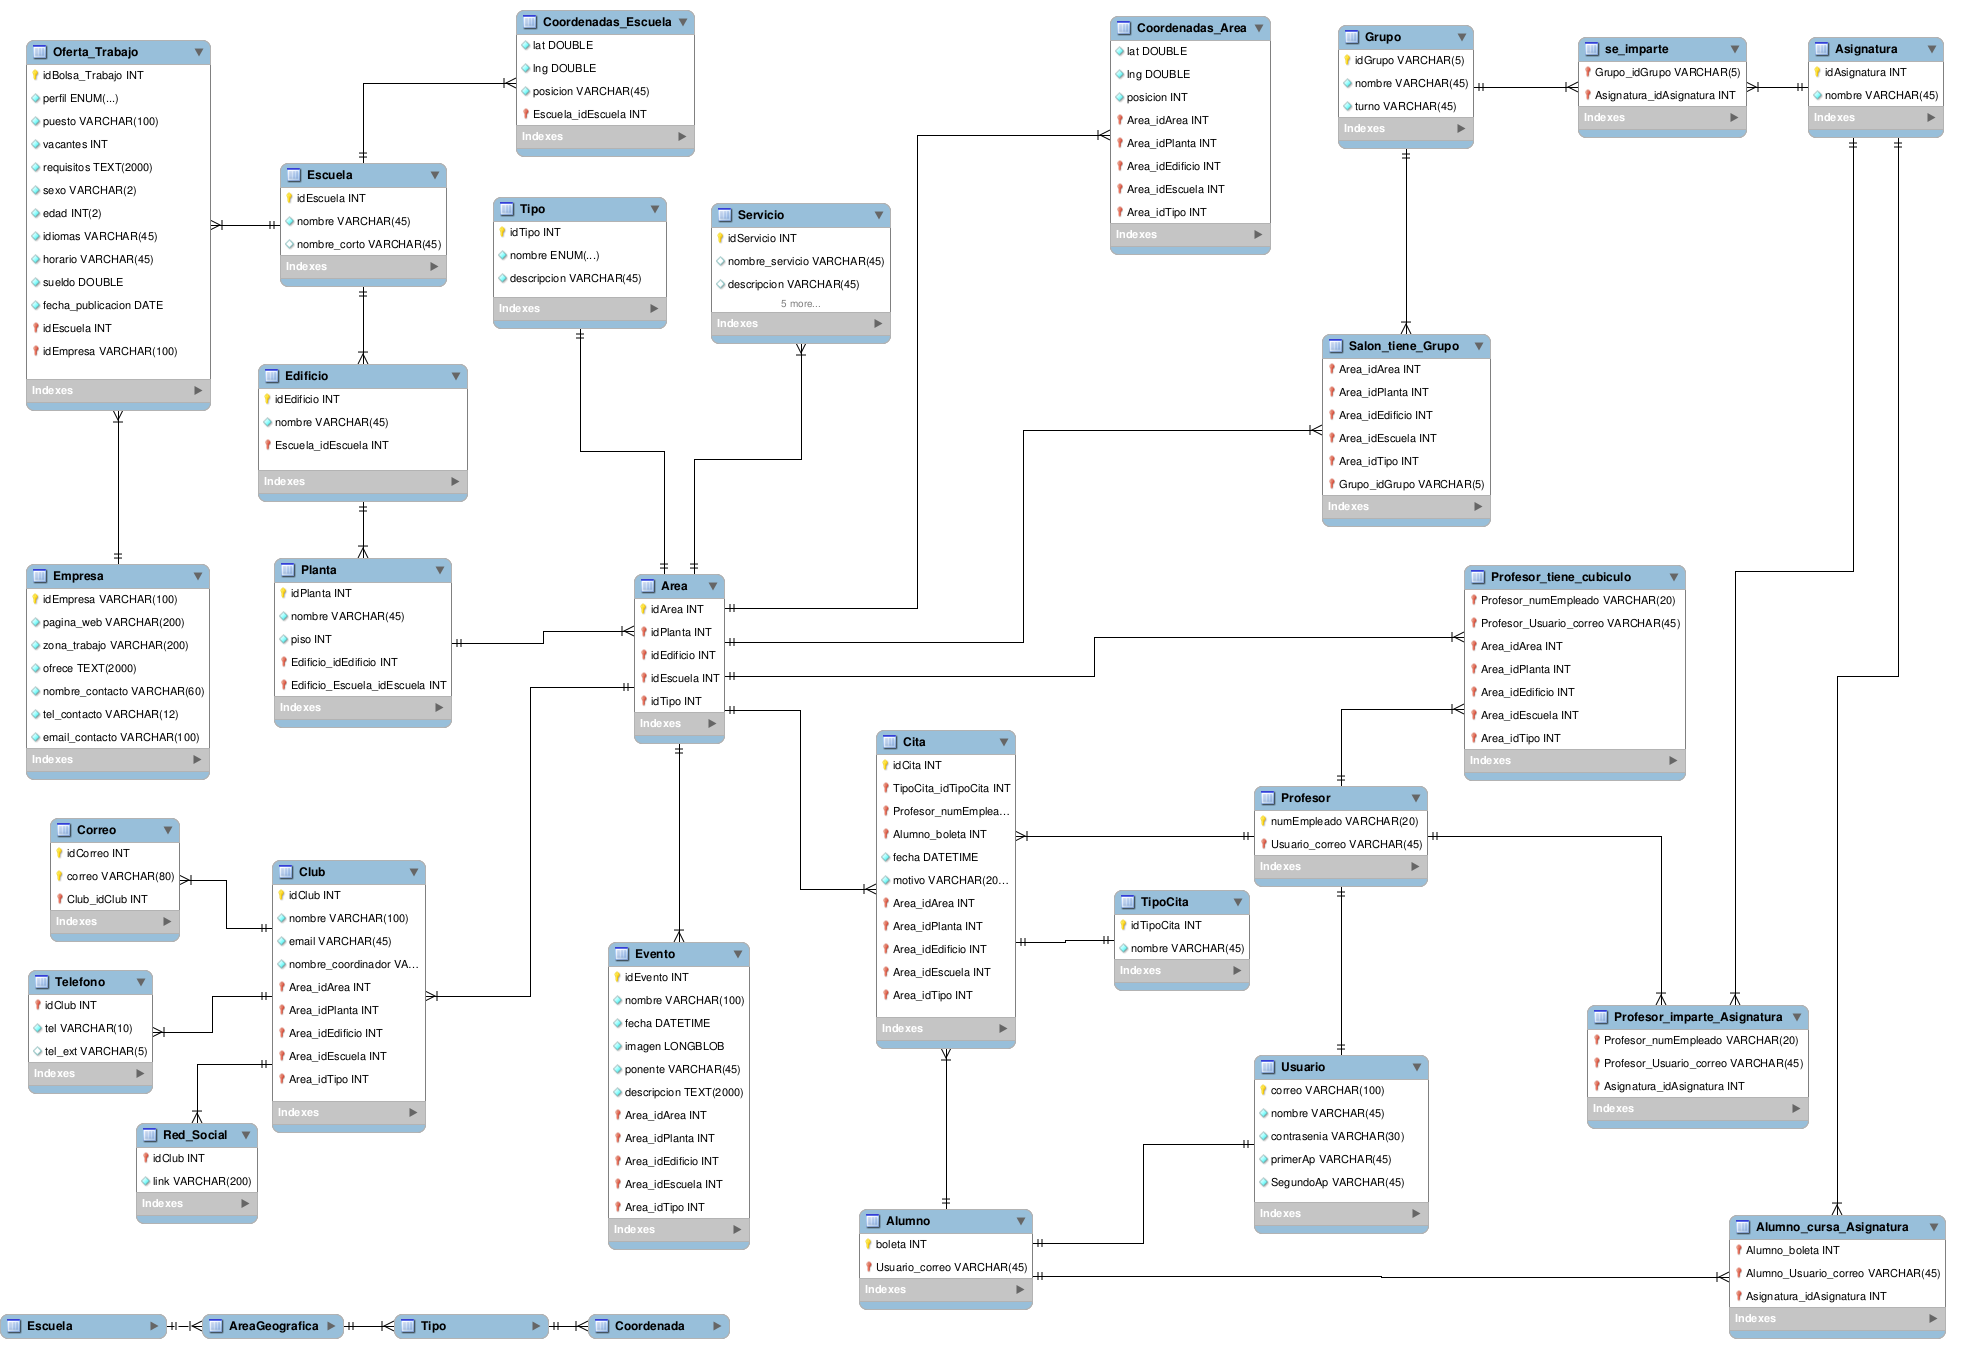
\includegraphics[width=1\textwidth]{images/baseDeDatos}
		%\caption{Diseño de la Base de Datos.}
		\caption{Diseño inconcluso de la base de datos.}
	\end{figure}

%=========================================================
%                                                              BIBLIOGRAFIA.
%=========================================================

\cfinput{bibliografia/bibliografia}

% FIN DEL DOCUMENTO.
\end{document}
